\section{Failure Analysis and Yield Improvement}

\subsection{Initial Observation}
The first production lots showed $\sim$65\% yield. Wafer test was dominated by \textbf{Pause Refresh Fail (Bin5)}. Defects appeared as uniformly scattered single-bit errors across the wafer (weak clustering, no edge/line signature). Storage-node capacitance met spec; SEM cross-sections at failed cells revealed no structural anomaly. Other CDs/films/electricals were within spec.

\begin{figure}[t]
  \centering
  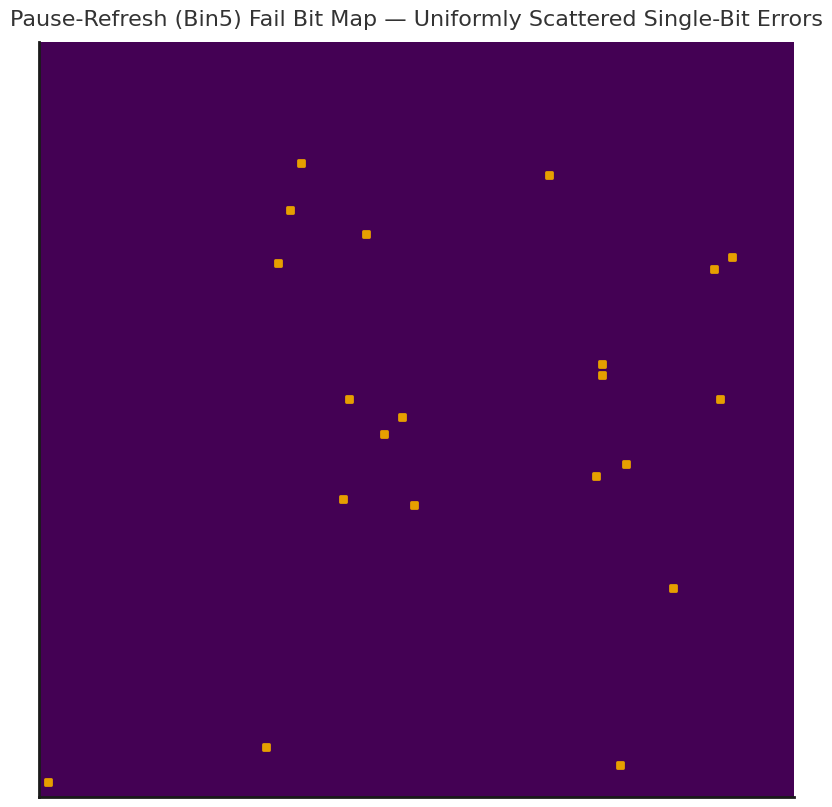
\includegraphics[width=\columnwidth]{fail_bitmap_bin5}
  \caption{Typical fail bit map under pause-refresh test (Bin5).
  Uniformly scattered single-bit errors are observed without edge/line signatures.}
  \label{fig:fail_bitmap}
\end{figure}

\subsection{Hypothesis (Failure Model)}
Directly measurable leakages were normal, suggesting a subtle leakage path. We hypothesized increased leakage at the \textbf{storage-node contact $n^+/p^-$ junction}. After gate etch, a remnant gate oxide on S/D active is repeatedly exposed to resist-stripping \emph{ashing} during multiple LDD steps. Cumulative plasma damage makes the oxide locally porous and can extend damage into the diffusion, creating minute leakage paths. This explains random single-bit distribution without visible structural defects.

% === Storage-node contact n+/p- leakage (TikZ) ===
% === Fig.2 Storage-node contact n+/p- leakage (pure TikZ, minimal IEEE style) ===
\begin{figure}[t]
\centering
\begin{tikzpicture}[x=1cm,y=1cm,line cap=round,line join=round]
  % 色(グレースケール)
  \def\colILD{black!7}    % ILD淡グレー
  \def\colSub{black!4}    % p-基板の淡グレー
  \def\colDiff{black!20}  % n+拡散
  \def\colLOCOS{black!20} % LOCOS輪郭
  \def\colMetal{black!60} % 金属プラグ

  % キャンバス範囲
  \path (-4.8,-2.4) rectangle (6.0,2.0);

  % ---- ILD(上部帯)----
  \fill[\colILD] (-4.8,0) rectangle (6.0,2.0);
  \node[anchor=east, font=\scriptsize] at (5.7,1.75) {ILD};

  % ---- 基板と表面 ----
  \fill[\colSub] (-4.8,-2.4) rectangle (6.0,0);
  \draw (-4.8,0) -- (6.0,0);
  \node[anchor=west, font=\scriptsize] at (-4.5,-2.1) {$p^{-}$ substrate};

  % ---- LOCOS(右側の鳥のくちばし風プロファイル)----
  \draw[\colLOCOS, line width=0.8pt]
    (1.8,0.20) .. controls (3.0,0.60) and (4.2,0.30) .. (5.2,0.20);

  % ---- n+拡散(ストレージ側)----
  \fill[\colDiff] ( -0.4,-1.1) rectangle (1.4,-0.4);
  \draw ( -0.4,-1.1) rectangle (1.4,-0.4);
  \node[font=\scriptsize] at (0.5,-0.75) {$n^{+}$};

  % ---- ストレージノード・コンタクトプラグ ----
  \fill[\colMetal] (0.35,0.00) rectangle (0.85,0.85);
  \draw (0.35,0.00) rectangle (0.85,0.85);

  % ---- 破線リークパス(コンタクト端→接合)----
  \draw[very thick, dashed] (0.60,0.85) -- (0.60,-0.18);
  \draw[very thick, dashed, -{Latex[length=2mm]}] (0.60,-0.18) -- (0.95,-0.80);
  \node[anchor=west, font=\scriptsize] at (1.05,-0.85) {leakage path};

  % ---- 注記(最小限)----
  \node[anchor=west, font=\scriptsize] at (-2.9,-0.15) {plasma/LDD-induced damage};
  \node[anchor=west, font=\scriptsize] at (-2.9,-0.85) {junction leakage increase};
\end{tikzpicture}
\caption{Schematic of storage-node contact (n$^+$/p$^-$) leakage.
Damage near the contact edge increases junction leakage, degrading retention.}
\label{fig:storage_contact}
\end{figure}

\subsection{Countermeasures}
\begin{itemize}
  \item \textbf{Process}: Replace resist stripping in LDD steps from plasma ashing to \textbf{wet stripping (sulfuric-based)} to eliminate plasma damage. 
  \item \textbf{Integration hygiene}: Confirm downstream photo cleanliness and avoid residue risks with the wet strip.
\end{itemize}

\subsection{Effectiveness}
Yield improved from $\sim$65\% to \textbf{$\sim$80\%}. Uniformly scattered single-bit fails decreased markedly. Burn-in and retention/reliability passed; the final recipe was fixed for volume production.

% === Yield-by-lot (step improvement at countermeasure) ===
\begin{figure}[t]
\centering
\pgfplotstableread[col sep=comma]{data/yield_lot.csv}\yieldtbl
\begin{tikzpicture}
\begin{axis}[
  width=\columnwidth, height=0.58\columnwidth,
  xlabel={Lot ID}, ylabel={Yield [\%]},
  ymin=50, ymax=95,
  xmin=0.5, xmax=12.5,
  grid=both,
  xtick=data,
  xticklabels from table={\yieldtbl}{lot},
  xticklabel style={rotate=45, anchor=east},
]
  % データ描画
  \addplot+[mark=*] table[x expr=\coordindex+1, y=yield]{\yieldtbl};

  % 対策境界: lot04とlot05の間
  \draw[dashed] (axis cs:4.5,50) -- (axis cs:4.5,95);
  \node[anchor=west, font=\footnotesize] at (axis cs:4.55,92)
    {Countermeasure};
\end{axis}
\end{tikzpicture}
\caption{Yield step improvement at the countermeasure boundary
between \texttt{lot04} and \texttt{lot05}. Yield jumps from $\sim$62--63\% 
(lot01--lot04) to $\sim$82--84\% (lot05 onward) after changing 
LDD resist stripping from ashing to wet stripping.}
\label{fig:yield}
\end{figure}
